\documentclass[tikz,border=8pt]{standalone}
% Shared look for every TikZ diagram. Load with \input{../../tools/tikz-style.tex}
\usepackage[T1]{fontenc}
\usepackage{lmodern}
\renewcommand{\sfdefault}{lmr}  % diagrams use the same serif as the text
\usetikzlibrary{arrows.meta, positioning, shapes.geometric, calc, fit, backgrounds}
\definecolor{cblue}{HTML}{4C78A8}
\definecolor{corange}{HTML}{F58518}
\definecolor{cgreen}{HTML}{54A24B}
\definecolor{cred}{HTML}{E45756}
\definecolor{cpurple}{HTML}{B279A2}
\definecolor{cgrey}{HTML}{6B6B6B}
\tikzset{
  every picture/.style={font=\sffamily, line width=1.2pt},
  box/.style={draw=#1, fill=#1!12, rounded corners=4pt, align=center, inner sep=7pt, minimum height=1.1cm},
  box/.default=cgrey,
  arrow/.style={-{Stealth[length=3mm]}, draw=cgrey, line width=1.4pt},
  title/.style={font=\sffamily\bfseries\Large},
  note/.style={font=\sffamily\small, text=cgrey, align=center},
}
\AtBeginDocument{\hyphenpenalty=10000 \exhyphenpenalty=10000}

% Odometry from (2, 1, 30 deg) to (2.249, 1.409, 87.3 deg) as turn, drive, turn: rot1 = 0.500 rad, trans = 0.479 m,
% rot2 = 0.500 rad. The robot really drove the dashed arc; the three steps reach the same pose.
\begin{document}
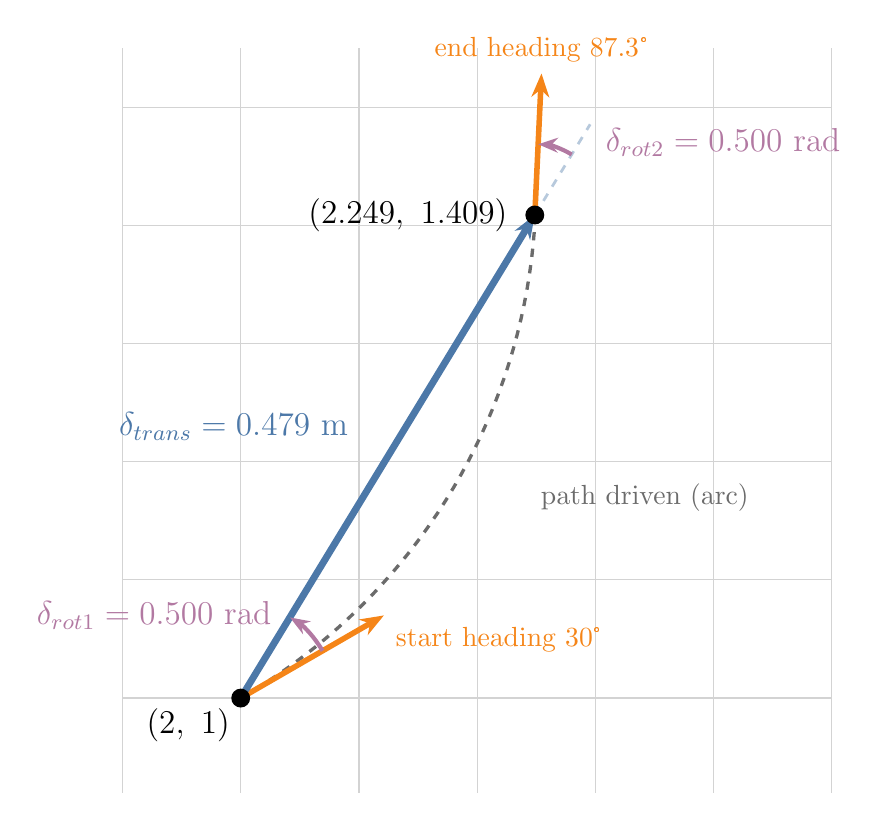
\begin{tikzpicture}[scale=15, every node/.append style={font=\large}]
  \coordinate (A) at (2,1); \coordinate (B) at (2.249,1.409);
  \draw[cgrey!30, line width=0.4pt] (1.9,0.92) grid[step=0.1] (2.5,1.55);
  \draw[cgrey, dashed, line width=1.2pt] plot[domain=0.5236:1.5236, samples=40] ({1.75+0.5*sin(\x r)}, {1.433-0.5*cos(\x r)});
  \node[cgrey, font=\normalsize, anchor=west] at (2.245,1.17) {path driven (arc)};
  % start heading and chord
  \draw[-{Stealth[length=3mm]}, corange, line width=2pt] (A) -- ++(30:0.14) node[below right, font=\normalsize] {start heading 30°};
  \draw[-{Stealth[length=3mm]}, cblue, line width=2.5pt] (A) -- (B);
  \node[cblue, anchor=east] at (2.1,1.23) {$\delta_{\text{trans}} = 0.479$ m};
  \draw[cpurple, line width=1.5pt, -{Stealth[length=2.5mm]}] ($(A)+(30:0.08)$) arc (30:58.6:0.08);
  \node[cpurple, anchor=east] at (2.035,1.07) {$\delta_{\text{rot1}} = 0.500$ rad};
  % end heading
  \draw[cblue!40, dashed, line width=1pt] (B) -- ++(58.6:0.09);
  \draw[-{Stealth[length=3mm]}, corange, line width=2pt] (B) -- ++(87.3:0.12) node[above, font=\normalsize] {end heading 87.3°};
  \draw[cpurple, line width=1.5pt, -{Stealth[length=2.5mm]}] ($(B)+(58.6:0.06)$) arc (58.6:87.3:0.06);
  \node[cpurple, right] at (2.3,1.47) {$\delta_{\text{rot2}} = 0.500$ rad};
  \fill[black] (A) circle (0.008) node[below left] {$(2,\ 1)$};
  \fill[black] (B) circle (0.008) node[left=6pt] {$(2.249,\ 1.409)$};
\end{tikzpicture}
\end{document}
